\documentclass[1p]{elsarticle_modified}
%\bibliographystyle{elsarticle-num}

%\usepackage[colorlinks]{hyperref}
%\usepackage{abbrmath_seonhwa} %\Abb, \Ascr, \Acal ,\Abf, \Afrak
\usepackage{amsfonts}
\usepackage{amssymb}
\usepackage{amsmath}
\usepackage{amsthm}
\usepackage{scalefnt}
\usepackage{amsbsy}
\usepackage{kotex}
\usepackage{caption}
\usepackage{subfig}
\usepackage{color}
\usepackage{graphicx}
\usepackage{xcolor} %% white, black, red, green, blue, cyan, magenta, yellow
\usepackage{float}
\usepackage{setspace}
\usepackage{hyperref}

\usepackage{tikz}
\usetikzlibrary{arrows}

\usepackage{multirow}
\usepackage{array} % fixed length table
\usepackage{hhline}

%%%%%%%%%%%%%%%%%%%%%
\makeatletter
\renewcommand*\env@matrix[1][\arraystretch]{%
	\edef\arraystretch{#1}%
	\hskip -\arraycolsep
	\let\@ifnextchar\new@ifnextchar
	\array{*\c@MaxMatrixCols c}}
\makeatother %https://tex.stackexchange.com/questions/14071/how-can-i-increase-the-line-spacing-in-a-matrix
%%%%%%%%%%%%%%%

\usepackage[normalem]{ulem}

\newcommand{\msout}[1]{\ifmmode\text{\sout{\ensuremath{#1}}}\else\sout{#1}\fi}
%SOURCE: \msout is \stkout macro in https://tex.stackexchange.com/questions/20609/strikeout-in-math-mode

\newcommand{\cancel}[1]{
	\ifmmode
	{\color{red}\msout{#1}}
	\else
	{\color{red}\sout{#1}}
	\fi
}

\newcommand{\add}[1]{
	{\color{blue}\uwave{#1}}
}

\newcommand{\replace}[2]{
	\ifmmode
	{\color{red}\msout{#1}}{\color{blue}\uwave{#2}}
	\else
	{\color{red}\sout{#1}}{\color{blue}\uwave{#2}}
	\fi
}

\newcommand{\Sol}{\mathcal{S}} %segment
\newcommand{\D}{D} %diagram
\newcommand{\A}{\mathcal{A}} %arc


%%%%%%%%%%%%%%%%%%%%%%%%%%%%%5 test

\def\sl{\operatorname{\textup{SL}}(2,\Cbb)}
\def\psl{\operatorname{\textup{PSL}}(2,\Cbb)}
\def\quan{\mkern 1mu \triangleright \mkern 1mu}

\theoremstyle{definition}
\newtheorem{thm}{Theorem}[section]
\newtheorem{prop}[thm]{Proposition}
\newtheorem{lem}[thm]{Lemma}
\newtheorem{ques}[thm]{Question}
\newtheorem{cor}[thm]{Corollary}
\newtheorem{defn}[thm]{Definition}
\newtheorem{exam}[thm]{Example}
\newtheorem{rmk}[thm]{Remark}
\newtheorem{alg}[thm]{Algorithm}

\newcommand{\I}{\sqrt{-1}}
\begin{document}

%\begin{frontmatter}
%
%\title{Boundary parabolic representations of knots up to 8 crossings}
%
%%% Group authors per affiliation:
%\author{Yunhi Cho} 
%\address{Department of Mathematics, University of Seoul, Seoul, Korea}
%\ead{yhcho@uos.ac.kr}
%
%
%\author{Seonhwa Kim} %\fnref{s_kim}}
%\address{Center for Geometry and Physics, Institute for Basic Science, Pohang, 37673, Korea}
%\ead{ryeona17@ibs.re.kr}
%
%\author{Hyuk Kim}
%\address{Department of Mathematical Sciences, Seoul National University, Seoul 08826, Korea}
%\ead{hyukkim@snu.ac.kr}
%
%\author{Seokbeom Yoon}
%\address{Department of Mathematical Sciences, Seoul National University, Seoul, 08826,  Korea}
%\ead{sbyoon15@snu.ac.kr}
%
%\begin{abstract}
%We find all boundary parabolic representation of knots up to 8 crossings.
%
%\end{abstract}
%\begin{keyword}
%    \MSC[2010] 57M25 
%\end{keyword}
%
%\end{frontmatter}

%\linenumbers
%\tableofcontents
%
\newcommand\colored[1]{\textcolor{white}{\rule[-0.35ex]{0.8em}{1.4ex}}\kern-0.8em\color{red} #1}%
%\newcommand\colored[1]{\textcolor{white}{ #1}\kern-2.17ex	\textcolor{white}{ #1}\kern-1.81ex	\textcolor{white}{ #1}\kern-2.15ex\color{red}#1	}

{\Large $\underline{12a_{0631}~(K12a_{0631})}$}

\setlength{\tabcolsep}{10pt}
\renewcommand{\arraystretch}{1.6}
\vspace{1cm}\begin{tabular}{m{100pt}>{\centering\arraybackslash}m{274pt}}
\multirow{5}{120pt}{
	\centering
	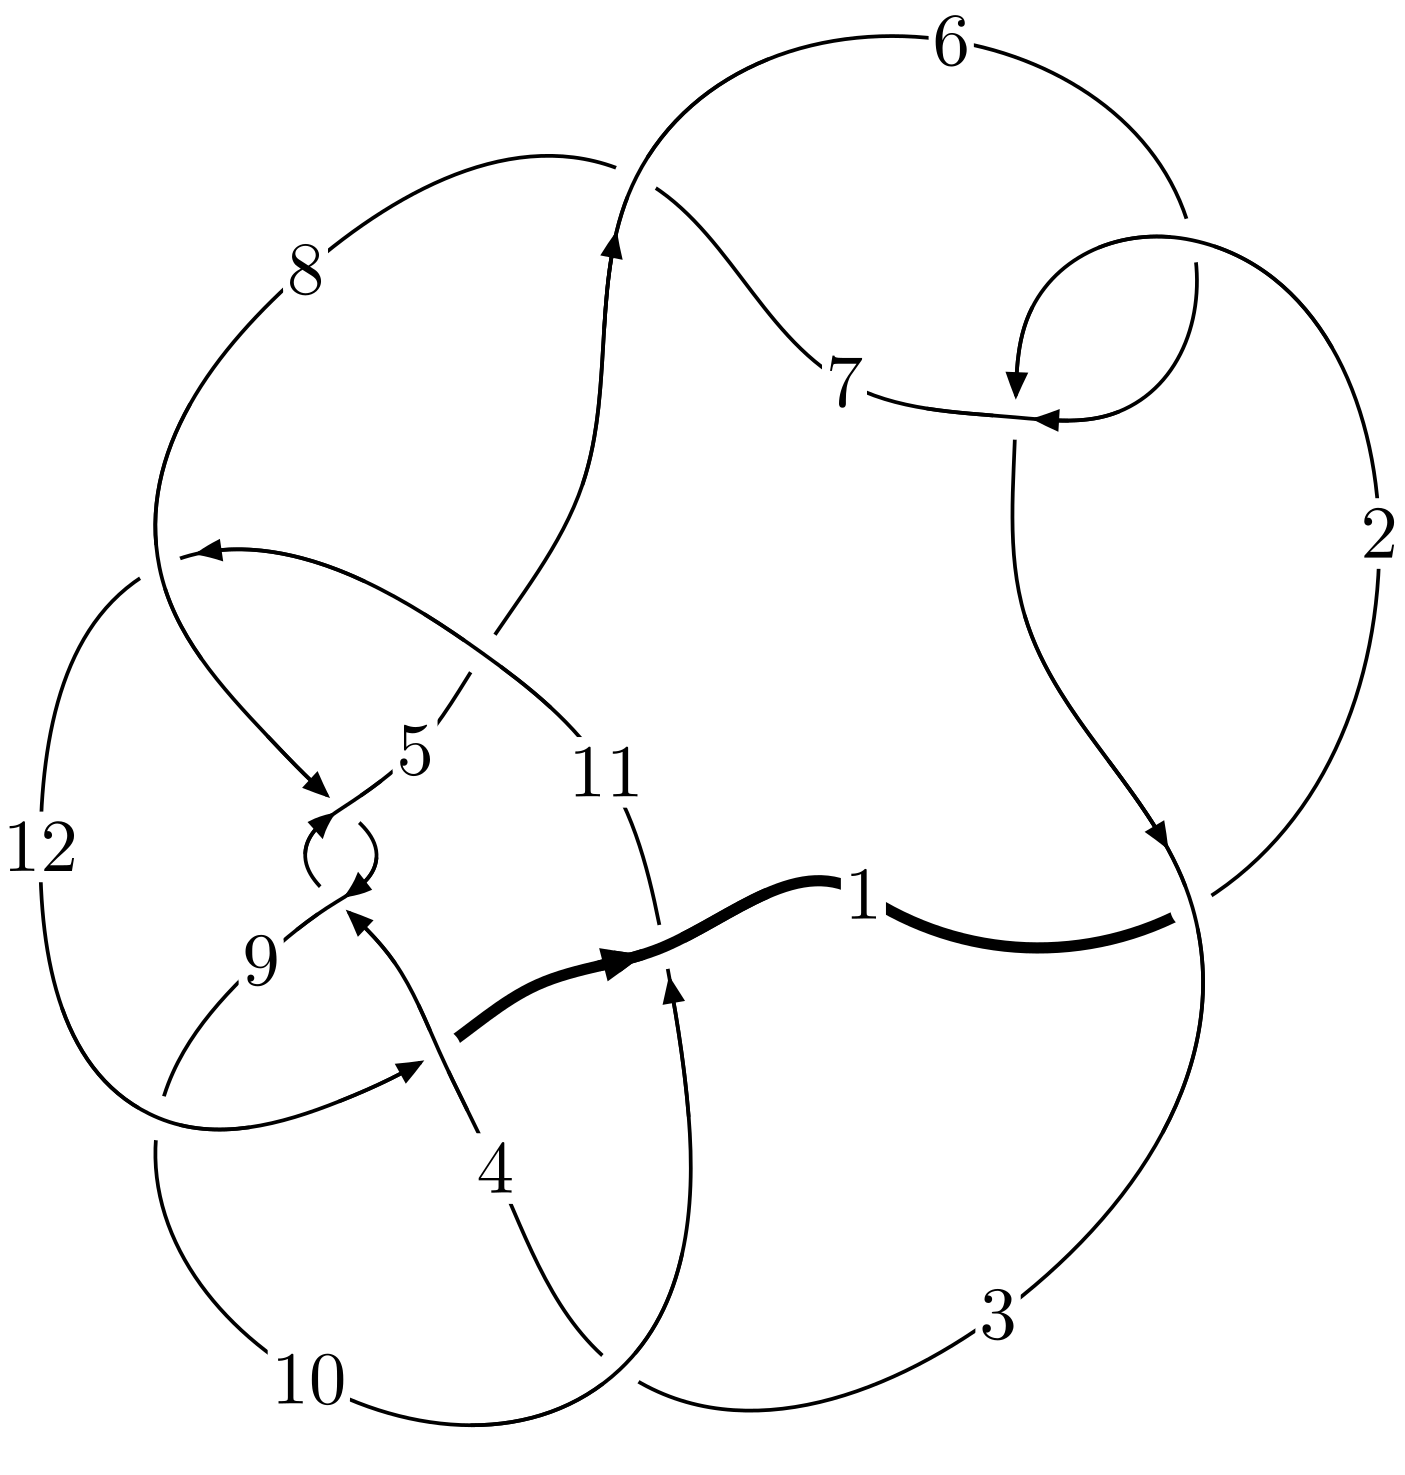
\includegraphics[width=112pt]{../../../GIT/diagram.site/Diagrams/png/1432_12a_0631.png}\\
\ \ \ A knot diagram\footnotemark}&
\allowdisplaybreaks
\textbf{Linearized knot diagam} \\
\cline{2-2}
 &
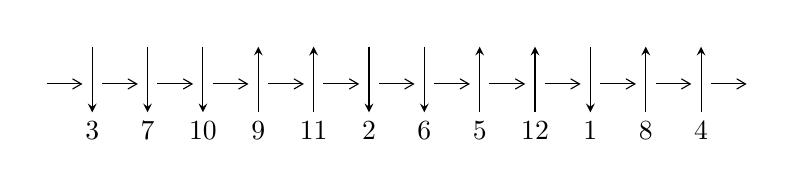
\begin{tikzpicture}[x=20pt, y=17pt]
	% nodes
	\node (C0) at (0, 0) {};
	\node (C1) at (1, 0) {};
	\node (C1U) at (1, +1) {};
	\node (C1D) at (1, -1) {3};

	\node (C2) at (2, 0) {};
	\node (C2U) at (2, +1) {};
	\node (C2D) at (2, -1) {7};

	\node (C3) at (3, 0) {};
	\node (C3U) at (3, +1) {};
	\node (C3D) at (3, -1) {10};

	\node (C4) at (4, 0) {};
	\node (C4U) at (4, +1) {};
	\node (C4D) at (4, -1) {9};

	\node (C5) at (5, 0) {};
	\node (C5U) at (5, +1) {};
	\node (C5D) at (5, -1) {11};

	\node (C6) at (6, 0) {};
	\node (C6U) at (6, +1) {};
	\node (C6D) at (6, -1) {2};

	\node (C7) at (7, 0) {};
	\node (C7U) at (7, +1) {};
	\node (C7D) at (7, -1) {6};

	\node (C8) at (8, 0) {};
	\node (C8U) at (8, +1) {};
	\node (C8D) at (8, -1) {5};

	\node (C9) at (9, 0) {};
	\node (C9U) at (9, +1) {};
	\node (C9D) at (9, -1) {12};

	\node (C10) at (10, 0) {};
	\node (C10U) at (10, +1) {};
	\node (C10D) at (10, -1) {1};

	\node (C11) at (11, 0) {};
	\node (C11U) at (11, +1) {};
	\node (C11D) at (11, -1) {8};

	\node (C12) at (12, 0) {};
	\node (C12U) at (12, +1) {};
	\node (C12D) at (12, -1) {4};
	\node (C13) at (13, 0) {};

	% arrows
	\draw[->,>={angle 60}]
	(C0) edge (C1) (C1) edge (C2) (C2) edge (C3) (C3) edge (C4) (C4) edge (C5) (C5) edge (C6) (C6) edge (C7) (C7) edge (C8) (C8) edge (C9) (C9) edge (C10) (C10) edge (C11) (C11) edge (C12) (C12) edge (C13) ;	\draw[->,>=stealth]
	(C1U) edge (C1D) (C2U) edge (C2D) (C3U) edge (C3D) (C4D) edge (C4U) (C5D) edge (C5U) (C6U) edge (C6D) (C7U) edge (C7D) (C8D) edge (C8U) (C9D) edge (C9U) (C10U) edge (C10D) (C11D) edge (C11U) (C12D) edge (C12U) ;
	\end{tikzpicture} \\
\hhline{~~} \\& 
\textbf{Solving Sequence} \\ \cline{2-2} 
 &
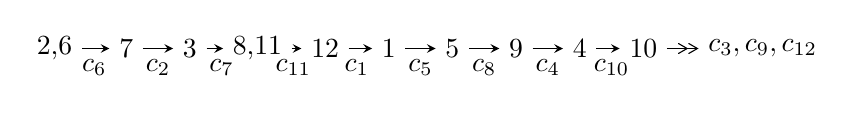
\begin{tikzpicture}[x=23pt, y=7pt]
	% node
	\node (A0) at (-1/8, 0) {2,6};
	\node (A1) at (1, 0) {7};
	\node (A2) at (2, 0) {3};
	\node (A3) at (49/16, 0) {8,11};
	\node (A4) at (33/8, 0) {12};
	\node (A5) at (41/8, 0) {1};
	\node (A6) at (49/8, 0) {5};
	\node (A7) at (57/8, 0) {9};
	\node (A8) at (65/8, 0) {4};
	\node (A9) at (73/8, 0) {10};
	\node (C1) at (1/2, -1) {$c_{6}$};
	\node (C2) at (3/2, -1) {$c_{2}$};
	\node (C3) at (5/2, -1) {$c_{7}$};
	\node (C4) at (29/8, -1) {$c_{11}$};
	\node (C5) at (37/8, -1) {$c_{1}$};
	\node (C6) at (45/8, -1) {$c_{5}$};
	\node (C7) at (53/8, -1) {$c_{8}$};
	\node (C8) at (61/8, -1) {$c_{4}$};
	\node (C9) at (69/8, -1) {$c_{10}$};
	\node (A10) at (11, 0) {$c_{3},c_{9},c_{12}$};

	% edge
	\draw[->,>=stealth]	
	(A0) edge (A1) (A1) edge (A2) (A2) edge (A3) (A3) edge (A4) (A4) edge (A5) (A5) edge (A6) (A6) edge (A7) (A7) edge (A8) (A8) edge (A9) ;
	\draw[->>,>={angle 60}]	
	(A9) edge (A10);
\end{tikzpicture} \\ 

\end{tabular} \\

\footnotetext{
The image of knot diagram is generated by the software ``\textbf{Draw programme}" developed by Andrew Bartholomew(\url{http://www.layer8.co.uk/maths/draw/index.htm\#Running-draw}), where we modified some parts for our purpose(\url{https://github.com/CATsTAILs/LinksPainter}).
}\phantom \\ \newline 
\centering \textbf{Ideals for irreducible components\footnotemark of $X_{\text{par}}$} 
 
\begin{align*}
I^u_{1}&=\langle 
-1.55586\times10^{199} u^{136}-3.48558\times10^{199} u^{135}+\cdots+7.08230\times10^{199} b-2.19097\times10^{201},\\
\phantom{I^u_{1}}&\phantom{= \langle  }-3.62369\times10^{200} u^{136}+5.95737\times10^{199} u^{135}+\cdots+9.20699\times10^{200} a-4.72404\times10^{202},\\
\phantom{I^u_{1}}&\phantom{= \langle  }u^{137}-20 u^{135}+\cdots+8 u+13\rangle \\
I^u_{2}&=\langle 
-2 u^{24}-2 u^{23}+\cdots+b+3 u,\;411 u^{24}+715 u^{23}+\cdots+29 a-1052,\;u^{25}+u^{24}+\cdots-9 u^2+1\rangle \\
\\
\end{align*}
\raggedright * 2 irreducible components of $\dim_{\mathbb{C}}=0$, with total 162 representations.\\
\footnotetext{All coefficients of polynomials are rational numbers. But the coefficients are sometimes approximated in decimal forms when there is not enough margin.}
\newpage
\renewcommand{\arraystretch}{1}
\centering \section*{I. $I^u_{1}= \langle -1.56\times10^{199} u^{136}-3.49\times10^{199} u^{135}+\cdots+7.08\times10^{199} b-2.19\times10^{201},\;-3.62\times10^{200} u^{136}+5.96\times10^{199} u^{135}+\cdots+9.21\times10^{200} a-4.72\times10^{202},\;u^{137}-20 u^{135}+\cdots+8 u+13 \rangle$}
\flushleft \textbf{(i) Arc colorings}\\
\begin{tabular}{m{7pt} m{180pt} m{7pt} m{180pt} }
\flushright $a_{2}=$&$\begin{pmatrix}0\\u\end{pmatrix}$ \\
\flushright $a_{6}=$&$\begin{pmatrix}1\\0\end{pmatrix}$ \\
\flushright $a_{7}=$&$\begin{pmatrix}1\\u^2\end{pmatrix}$ \\
\flushright $a_{3}=$&$\begin{pmatrix}- u\\- u^3+u\end{pmatrix}$ \\
\flushright $a_{8}=$&$\begin{pmatrix}- u^2+1\\u^2\end{pmatrix}$ \\
\flushright $a_{11}=$&$\begin{pmatrix}0.393580 u^{136}-0.0647048 u^{135}+\cdots-72.5869 u+51.3092\\0.219683 u^{136}+0.492153 u^{135}+\cdots-16.7611 u+30.9359\end{pmatrix}$ \\
\flushright $a_{12}=$&$\begin{pmatrix}0.624416 u^{136}-1.58638 u^{135}+\cdots-71.2059 u+68.4912\\1.42220 u^{136}+0.528391 u^{135}+\cdots-23.5112 u+50.2466\end{pmatrix}$ \\
\flushright $a_{1}=$&$\begin{pmatrix}u^3\\u^5- u^3+u\end{pmatrix}$ \\
\flushright $a_{5}=$&$\begin{pmatrix}5.56418 u^{136}-4.23778 u^{135}+\cdots-98.6052 u+66.8624\\3.90303 u^{136}-4.04280 u^{135}+\cdots-37.9656 u+104.599\end{pmatrix}$ \\
\flushright $a_{9}=$&$\begin{pmatrix}-0.540857 u^{136}+1.45019 u^{135}+\cdots+13.5778 u-12.5870\\-2.27532 u^{136}-0.201414 u^{135}+\cdots+54.9112 u-22.6952\end{pmatrix}$ \\
\flushright $a_{4}=$&$\begin{pmatrix}4.41963 u^{136}-3.59377 u^{135}+\cdots-71.2216 u+92.7479\\4.18373 u^{136}-3.47970 u^{135}+\cdots-56.9236 u+81.5572\end{pmatrix}$ \\
\flushright $a_{10}=$&$\begin{pmatrix}0.208814 u^{136}-0.757186 u^{135}+\cdots-69.1192 u+57.1447\\0.453845 u^{136}+0.907411 u^{135}+\cdots-0.585492 u+26.8148\end{pmatrix}$\\&\end{tabular}
\flushleft \textbf{(ii) Obstruction class $= -1$}\\~\\
\flushleft \textbf{(iii) Cusp Shapes $= -2.68992 u^{136}+6.00496 u^{135}+\cdots-46.6040 u-120.851$}\\~\\
\newpage\renewcommand{\arraystretch}{1}
\flushleft \textbf{(iv) u-Polynomials at the component}\newline \\
\begin{tabular}{m{50pt}|m{274pt}}
Crossings & \hspace{64pt}u-Polynomials at each crossing \\
\hline $$\begin{aligned}c_{1},c_{7}\end{aligned}$$&$\begin{aligned}
&u^{137}+40 u^{136}+\cdots+4042 u+169
\end{aligned}$\\
\hline $$\begin{aligned}c_{2},c_{6}\end{aligned}$$&$\begin{aligned}
&u^{137}-20 u^{135}+\cdots+8 u+13
\end{aligned}$\\
\hline $$\begin{aligned}c_{3}\end{aligned}$$&$\begin{aligned}
&u^{137}+2 u^{136}+\cdots-31644 u+3869
\end{aligned}$\\
\hline $$\begin{aligned}c_{4},c_{8}\end{aligned}$$&$\begin{aligned}
&u^{137}+6 u^{136}+\cdots+60 u+2
\end{aligned}$\\
\hline $$\begin{aligned}c_{5}\end{aligned}$$&$\begin{aligned}
&u^{137}+u^{136}+\cdots+11 u+1
\end{aligned}$\\
\hline $$\begin{aligned}c_{9}\end{aligned}$$&$\begin{aligned}
&u^{137}-12 u^{136}+\cdots+48 u+1
\end{aligned}$\\
\hline $$\begin{aligned}c_{10}\end{aligned}$$&$\begin{aligned}
&u^{137}+9 u^{136}+\cdots+32 u-128
\end{aligned}$\\
\hline $$\begin{aligned}c_{11}\end{aligned}$$&$\begin{aligned}
&u^{137}+u^{136}+\cdots+760 u+7
\end{aligned}$\\
\hline $$\begin{aligned}c_{12}\end{aligned}$$&$\begin{aligned}
&u^{137}+9 u^{136}+\cdots+55158 u+5036
\end{aligned}$\\
\hline
\end{tabular}\\~\\
\newpage\renewcommand{\arraystretch}{1}
\flushleft \textbf{(v) Riley Polynomials at the component}\newline \\
\begin{tabular}{m{50pt}|m{274pt}}
Crossings & \hspace{64pt}Riley Polynomials at each crossing \\
\hline $$\begin{aligned}c_{1},c_{7}\end{aligned}$$&$\begin{aligned}
&y^{137}+120 y^{136}+\cdots+779962 y-28561
\end{aligned}$\\
\hline $$\begin{aligned}c_{2},c_{6}\end{aligned}$$&$\begin{aligned}
&y^{137}-40 y^{136}+\cdots+4042 y-169
\end{aligned}$\\
\hline $$\begin{aligned}c_{3}\end{aligned}$$&$\begin{aligned}
&y^{137}+36 y^{136}+\cdots-513688022 y-14969161
\end{aligned}$\\
\hline $$\begin{aligned}c_{4},c_{8}\end{aligned}$$&$\begin{aligned}
&y^{137}+100 y^{136}+\cdots-848 y-4
\end{aligned}$\\
\hline $$\begin{aligned}c_{5}\end{aligned}$$&$\begin{aligned}
&y^{137}-3 y^{136}+\cdots-191 y-1
\end{aligned}$\\
\hline $$\begin{aligned}c_{9}\end{aligned}$$&$\begin{aligned}
&y^{137}+12 y^{136}+\cdots-696 y-1
\end{aligned}$\\
\hline $$\begin{aligned}c_{10}\end{aligned}$$&$\begin{aligned}
&y^{137}+21 y^{136}+\cdots+152576 y-16384
\end{aligned}$\\
\hline $$\begin{aligned}c_{11}\end{aligned}$$&$\begin{aligned}
&y^{137}-13 y^{136}+\cdots+530448 y-49
\end{aligned}$\\
\hline $$\begin{aligned}c_{12}\end{aligned}$$&$\begin{aligned}
&y^{137}+35 y^{136}+\cdots-1685724212 y-25361296
\end{aligned}$\\
\hline
\end{tabular}\\~\\
\newpage\flushleft \textbf{(vi) Complex Volumes and Cusp Shapes}
$$\begin{array}{c|c|c}  
\text{Solutions to }I^u_{1}& \I (\text{vol} + \sqrt{-1}CS) & \text{Cusp shape}\\
 \hline 
\begin{aligned}
u &= -0.950342 + 0.290973 I \\
a &= \phantom{-}0.93783 - 1.43485 I \\
b &= -0.91390 - 1.41574 I\end{aligned}
 & -6.41076 + 4.67038 I & \phantom{-0.000000 } 0 \\ \hline\begin{aligned}
u &= -0.950342 - 0.290973 I \\
a &= \phantom{-}0.93783 + 1.43485 I \\
b &= -0.91390 + 1.41574 I\end{aligned}
 & -6.41076 - 4.67038 I & \phantom{-0.000000 } 0 \\ \hline\begin{aligned}
u &= -1.001520 + 0.114802 I \\
a &= \phantom{-}1.62158 - 1.27980 I \\
b &= \phantom{-}0.085542 - 0.708863 I\end{aligned}
 & -5.96822 + 4.40940 I & \phantom{-0.000000 } 0 \\ \hline\begin{aligned}
u &= -1.001520 - 0.114802 I \\
a &= \phantom{-}1.62158 + 1.27980 I \\
b &= \phantom{-}0.085542 + 0.708863 I\end{aligned}
 & -5.96822 - 4.40940 I & \phantom{-0.000000 } 0 \\ \hline\begin{aligned}
u &= -0.909207 + 0.443165 I \\
a &= \phantom{-}0.530936 - 0.405342 I \\
b &= \phantom{-}0.330665 - 0.334576 I\end{aligned}
 & -1.89367 + 1.23105 I & \phantom{-0.000000 } 0 \\ \hline\begin{aligned}
u &= -0.909207 - 0.443165 I \\
a &= \phantom{-}0.530936 + 0.405342 I \\
b &= \phantom{-}0.330665 + 0.334576 I\end{aligned}
 & -1.89367 - 1.23105 I & \phantom{-0.000000 } 0 \\ \hline\begin{aligned}
u &= \phantom{-}0.956317 + 0.220620 I \\
a &= -0.931643 - 1.054290 I \\
b &= \phantom{-}0.591141 - 0.803215 I\end{aligned}
 & -2.78104 - 3.83969 I & \phantom{-0.000000 } 0 \\ \hline\begin{aligned}
u &= \phantom{-}0.956317 - 0.220620 I \\
a &= -0.931643 + 1.054290 I \\
b &= \phantom{-}0.591141 + 0.803215 I\end{aligned}
 & -2.78104 + 3.83969 I & \phantom{-0.000000 } 0 \\ \hline\begin{aligned}
u &= \phantom{-}1.007280 + 0.176412 I \\
a &= \phantom{-}0.008920 + 1.172450 I \\
b &= -0.75856 + 1.28902 I\end{aligned}
 & -6.99924 - 5.78107 I & \phantom{-0.000000 } 0 \\ \hline\begin{aligned}
u &= \phantom{-}1.007280 - 0.176412 I \\
a &= \phantom{-}0.008920 - 1.172450 I \\
b &= -0.75856 - 1.28902 I\end{aligned}
 & -6.99924 + 5.78107 I & \phantom{-0.000000 } 0\\
 \hline 
 \end{array}$$\newpage$$\begin{array}{c|c|c}  
\text{Solutions to }I^u_{1}& \I (\text{vol} + \sqrt{-1}CS) & \text{Cusp shape}\\
 \hline 
\begin{aligned}
u &= -0.935256 + 0.422309 I \\
a &= \phantom{-}0.582088 - 0.381280 I \\
b &= \phantom{-}0.117649 - 0.808197 I\end{aligned}
 & -1.81476 + 1.51215 I & \phantom{-0.000000 } 0 \\ \hline\begin{aligned}
u &= -0.935256 - 0.422309 I \\
a &= \phantom{-}0.582088 + 0.381280 I \\
b &= \phantom{-}0.117649 + 0.808197 I\end{aligned}
 & -1.81476 - 1.51215 I & \phantom{-0.000000 } 0 \\ \hline\begin{aligned}
u &= -0.791307 + 0.549429 I \\
a &= \phantom{-}0.446544 - 0.685802 I \\
b &= \phantom{-}0.266359 - 0.001806 I\end{aligned}
 & -1.92744 + 1.24860 I & \phantom{-0.000000 } 0 \\ \hline\begin{aligned}
u &= -0.791307 - 0.549429 I \\
a &= \phantom{-}0.446544 + 0.685802 I \\
b &= \phantom{-}0.266359 + 0.001806 I\end{aligned}
 & -1.92744 - 1.24860 I & \phantom{-0.000000 } 0 \\ \hline\begin{aligned}
u &= \phantom{-}0.894078 + 0.265913 I \\
a &= -1.65379 - 0.07115 I \\
b &= -0.283343 - 1.286370 I\end{aligned}
 & -6.60071 - 0.53295 I & \phantom{-0.000000 } 0 \\ \hline\begin{aligned}
u &= \phantom{-}0.894078 - 0.265913 I \\
a &= -1.65379 + 0.07115 I \\
b &= -0.283343 + 1.286370 I\end{aligned}
 & -6.60071 + 0.53295 I & \phantom{-0.000000 } 0 \\ \hline\begin{aligned}
u &= \phantom{-}0.794489 + 0.731554 I \\
a &= \phantom{-}1.62095 + 0.72026 I \\
b &= -1.375230 - 0.223785 I\end{aligned}
 & \phantom{-}2.71952 - 0.44182 I & \phantom{-0.000000 } 0 \\ \hline\begin{aligned}
u &= \phantom{-}0.794489 - 0.731554 I \\
a &= \phantom{-}1.62095 - 0.72026 I \\
b &= -1.375230 + 0.223785 I\end{aligned}
 & \phantom{-}2.71952 + 0.44182 I & \phantom{-0.000000 } 0 \\ \hline\begin{aligned}
u &= \phantom{-}0.782958 + 0.749202 I \\
a &= -1.65544 - 0.30724 I \\
b &= -0.0336307 + 0.0554863 I\end{aligned}
 & -0.37534 + 3.64365 I & \phantom{-0.000000 } 0 \\ \hline\begin{aligned}
u &= \phantom{-}0.782958 - 0.749202 I \\
a &= -1.65544 + 0.30724 I \\
b &= -0.0336307 - 0.0554863 I\end{aligned}
 & -0.37534 - 3.64365 I & \phantom{-0.000000 } 0\\
 \hline 
 \end{array}$$\newpage$$\begin{array}{c|c|c}  
\text{Solutions to }I^u_{1}& \I (\text{vol} + \sqrt{-1}CS) & \text{Cusp shape}\\
 \hline 
\begin{aligned}
u &= -0.768257 + 0.785459 I \\
a &= -0.99074 + 1.59719 I \\
b &= \phantom{-}1.41503 - 1.30206 I\end{aligned}
 & -0.73290 - 4.89341 I & \phantom{-0.000000 } 0 \\ \hline\begin{aligned}
u &= -0.768257 - 0.785459 I \\
a &= -0.99074 - 1.59719 I \\
b &= \phantom{-}1.41503 + 1.30206 I\end{aligned}
 & -0.73290 + 4.89341 I & \phantom{-0.000000 } 0 \\ \hline\begin{aligned}
u &= -1.098210 + 0.039739 I \\
a &= \phantom{-}0.000744 + 0.224690 I \\
b &= \phantom{-}0.429666 + 0.334160 I\end{aligned}
 & -2.38231 - 0.07495 I & \phantom{-0.000000 } 0 \\ \hline\begin{aligned}
u &= -1.098210 - 0.039739 I \\
a &= \phantom{-}0.000744 - 0.224690 I \\
b &= \phantom{-}0.429666 - 0.334160 I\end{aligned}
 & -2.38231 + 0.07495 I & \phantom{-0.000000 } 0 \\ \hline\begin{aligned}
u &= -1.014590 + 0.425663 I \\
a &= -1.130760 - 0.526430 I \\
b &= -0.263711 + 0.872601 I\end{aligned}
 & -5.56798 + 0.31097 I & \phantom{-0.000000 } 0 \\ \hline\begin{aligned}
u &= -1.014590 - 0.425663 I \\
a &= -1.130760 + 0.526430 I \\
b &= -0.263711 - 0.872601 I\end{aligned}
 & -5.56798 - 0.31097 I & \phantom{-0.000000 } 0 \\ \hline\begin{aligned}
u &= \phantom{-}1.084680 + 0.245425 I \\
a &= -0.373890 - 1.292780 I \\
b &= \phantom{-}0.599391 - 0.872750 I\end{aligned}
 & -2.80549 - 5.27118 I & \phantom{-0.000000 } 0 \\ \hline\begin{aligned}
u &= \phantom{-}1.084680 - 0.245425 I \\
a &= -0.373890 + 1.292780 I \\
b &= \phantom{-}0.599391 + 0.872750 I\end{aligned}
 & -2.80549 + 5.27118 I & \phantom{-0.000000 } 0 \\ \hline\begin{aligned}
u &= -0.885377 + 0.676654 I \\
a &= -1.39524 - 0.56773 I \\
b &= \phantom{-}0.207385 + 0.294997 I\end{aligned}
 & -2.12146 + 3.75084 I & \phantom{-0.000000 } 0 \\ \hline\begin{aligned}
u &= -0.885377 - 0.676654 I \\
a &= -1.39524 + 0.56773 I \\
b &= \phantom{-}0.207385 - 0.294997 I\end{aligned}
 & -2.12146 - 3.75084 I & \phantom{-0.000000 } 0\\
 \hline 
 \end{array}$$\newpage$$\begin{array}{c|c|c}  
\text{Solutions to }I^u_{1}& \I (\text{vol} + \sqrt{-1}CS) & \text{Cusp shape}\\
 \hline 
\begin{aligned}
u &= \phantom{-}0.986584 + 0.522645 I \\
a &= -0.537739 - 1.149890 I \\
b &= \phantom{-}0.128058 - 1.077410 I\end{aligned}
 & -3.61378 - 1.44795 I & \phantom{-0.000000 } 0 \\ \hline\begin{aligned}
u &= \phantom{-}0.986584 - 0.522645 I \\
a &= -0.537739 + 1.149890 I \\
b &= \phantom{-}0.128058 + 1.077410 I\end{aligned}
 & -3.61378 + 1.44795 I & \phantom{-0.000000 } 0 \\ \hline\begin{aligned}
u &= \phantom{-}0.048135 + 0.880536 I \\
a &= -0.493626 - 0.402684 I \\
b &= \phantom{-}0.622431 + 0.305290 I\end{aligned}
 & \phantom{-}2.56389 + 3.71181 I & \phantom{-0.000000 } 0 \\ \hline\begin{aligned}
u &= \phantom{-}0.048135 - 0.880536 I \\
a &= -0.493626 + 0.402684 I \\
b &= \phantom{-}0.622431 - 0.305290 I\end{aligned}
 & \phantom{-}2.56389 - 3.71181 I & \phantom{-0.000000 } 0 \\ \hline\begin{aligned}
u &= \phantom{-}0.709176 + 0.889402 I \\
a &= \phantom{-}1.060470 + 0.245934 I \\
b &= -0.938472 - 0.032551 I\end{aligned}
 & \phantom{-}4.44847 + 0.62496 I & \phantom{-0.000000 } 0 \\ \hline\begin{aligned}
u &= \phantom{-}0.709176 - 0.889402 I \\
a &= \phantom{-}1.060470 - 0.245934 I \\
b &= -0.938472 + 0.032551 I\end{aligned}
 & \phantom{-}4.44847 - 0.62496 I & \phantom{-0.000000 } 0 \\ \hline\begin{aligned}
u &= -0.804416 + 0.811717 I \\
a &= \phantom{-}1.58736 - 0.88904 I \\
b &= -0.984549 + 0.325999 I\end{aligned}
 & \phantom{-}3.76794 - 2.21552 I & \phantom{-0.000000 } 0 \\ \hline\begin{aligned}
u &= -0.804416 - 0.811717 I \\
a &= \phantom{-}1.58736 + 0.88904 I \\
b &= -0.984549 - 0.325999 I\end{aligned}
 & \phantom{-}3.76794 + 2.21552 I & \phantom{-0.000000 } 0 \\ \hline\begin{aligned}
u &= -0.738379 + 0.880183 I \\
a &= \phantom{-}0.924035 - 0.625755 I \\
b &= -0.917993 + 1.004520 I\end{aligned}
 & \phantom{-}4.78596 - 4.84103 I & \phantom{-0.000000 } 0 \\ \hline\begin{aligned}
u &= -0.738379 - 0.880183 I \\
a &= \phantom{-}0.924035 + 0.625755 I \\
b &= -0.917993 - 1.004520 I\end{aligned}
 & \phantom{-}4.78596 + 4.84103 I & \phantom{-0.000000 } 0\\
 \hline 
 \end{array}$$\newpage$$\begin{array}{c|c|c}  
\text{Solutions to }I^u_{1}& \I (\text{vol} + \sqrt{-1}CS) & \text{Cusp shape}\\
 \hline 
\begin{aligned}
u &= -1.101370 + 0.334392 I \\
a &= -0.630612 + 1.044650 I \\
b &= \phantom{-}0.77479 + 1.20521 I\end{aligned}
 & -6.0459 + 13.5824 I & \phantom{-0.000000 } 0 \\ \hline\begin{aligned}
u &= -1.101370 - 0.334392 I \\
a &= -0.630612 - 1.044650 I \\
b &= \phantom{-}0.77479 - 1.20521 I\end{aligned}
 & -6.0459 - 13.5824 I & \phantom{-0.000000 } 0 \\ \hline\begin{aligned}
u &= -0.878380 + 0.744243 I \\
a &= \phantom{-}0.802399 - 0.213731 I \\
b &= \phantom{-}0.056170 - 1.387260 I\end{aligned}
 & -1.91195 + 2.82674 I & \phantom{-0.000000 } 0 \\ \hline\begin{aligned}
u &= -0.878380 - 0.744243 I \\
a &= \phantom{-}0.802399 + 0.213731 I \\
b &= \phantom{-}0.056170 + 1.387260 I\end{aligned}
 & -1.91195 - 2.82674 I & \phantom{-0.000000 } 0 \\ \hline\begin{aligned}
u &= -0.078237 + 0.841438 I \\
a &= \phantom{-}0.582772 - 0.819572 I \\
b &= -0.762907 + 0.915721 I\end{aligned}
 & -2.58279 - 9.55814 I & \phantom{-0.000000 } 0 \\ \hline\begin{aligned}
u &= -0.078237 - 0.841438 I \\
a &= \phantom{-}0.582772 + 0.819572 I \\
b &= -0.762907 - 0.915721 I\end{aligned}
 & -2.58279 + 9.55814 I & \phantom{-0.000000 } 0 \\ \hline\begin{aligned}
u &= \phantom{-}1.139990 + 0.192620 I \\
a &= \phantom{-}0.790000 + 0.279063 I \\
b &= \phantom{-}0.397059 + 0.882263 I\end{aligned}
 & -6.90350 + 6.13066 I & \phantom{-0.000000 } 0 \\ \hline\begin{aligned}
u &= \phantom{-}1.139990 - 0.192620 I \\
a &= \phantom{-}0.790000 - 0.279063 I \\
b &= \phantom{-}0.397059 - 0.882263 I\end{aligned}
 & -6.90350 - 6.13066 I & \phantom{-0.000000 } 0 \\ \hline\begin{aligned}
u &= \phantom{-}1.110150 + 0.335786 I \\
a &= \phantom{-}0.356989 + 0.624780 I \\
b &= -0.655276 + 0.780506 I\end{aligned}
 & -1.03048 - 7.81260 I & \phantom{-0.000000 } 0 \\ \hline\begin{aligned}
u &= \phantom{-}1.110150 - 0.335786 I \\
a &= \phantom{-}0.356989 - 0.624780 I \\
b &= -0.655276 - 0.780506 I\end{aligned}
 & -1.03048 + 7.81260 I & \phantom{-0.000000 } 0\\
 \hline 
 \end{array}$$\newpage$$\begin{array}{c|c|c}  
\text{Solutions to }I^u_{1}& \I (\text{vol} + \sqrt{-1}CS) & \text{Cusp shape}\\
 \hline 
\begin{aligned}
u &= \phantom{-}0.867468 + 0.781275 I \\
a &= -2.35155 - 0.02698 I \\
b &= \phantom{-}1.10985 - 1.62312 I\end{aligned}
 & \phantom{-}5.18453 - 1.05366 I & \phantom{-0.000000 } 0 \\ \hline\begin{aligned}
u &= \phantom{-}0.867468 - 0.781275 I \\
a &= -2.35155 + 0.02698 I \\
b &= \phantom{-}1.10985 + 1.62312 I\end{aligned}
 & \phantom{-}5.18453 + 1.05366 I & \phantom{-0.000000 } 0 \\ \hline\begin{aligned}
u &= \phantom{-}0.813156 + 0.841912 I \\
a &= -1.35305 - 1.68742 I \\
b &= \phantom{-}1.49093 + 1.21883 I\end{aligned}
 & \phantom{-}0.78055 + 2.73858 I & \phantom{-0.000000 } 0 \\ \hline\begin{aligned}
u &= \phantom{-}0.813156 - 0.841912 I \\
a &= -1.35305 + 1.68742 I \\
b &= \phantom{-}1.49093 - 1.21883 I\end{aligned}
 & \phantom{-}0.78055 - 2.73858 I & \phantom{-0.000000 } 0 \\ \hline\begin{aligned}
u &= \phantom{-}0.861177 + 0.796914 I \\
a &= -1.47855 - 0.64041 I \\
b &= \phantom{-}1.093070 + 0.842656 I\end{aligned}
 & \phantom{-}2.85072 + 2.60130 I & \phantom{-0.000000 } 0 \\ \hline\begin{aligned}
u &= \phantom{-}0.861177 - 0.796914 I \\
a &= -1.47855 + 0.64041 I \\
b &= \phantom{-}1.093070 - 0.842656 I\end{aligned}
 & \phantom{-}2.85072 - 2.60130 I & \phantom{-0.000000 } 0 \\ \hline\begin{aligned}
u &= -0.853253 + 0.814086 I \\
a &= \phantom{-}2.46708 - 0.94612 I \\
b &= -1.97715 - 0.64182 I\end{aligned}
 & \phantom{-}3.79616 - 3.17397 I & \phantom{-0.000000 } 0 \\ \hline\begin{aligned}
u &= -0.853253 - 0.814086 I \\
a &= \phantom{-}2.46708 + 0.94612 I \\
b &= -1.97715 + 0.64182 I\end{aligned}
 & \phantom{-}3.79616 + 3.17397 I & \phantom{-0.000000 } 0 \\ \hline\begin{aligned}
u &= \phantom{-}0.862701 + 0.805862 I \\
a &= \phantom{-}1.68281 - 0.06727 I \\
b &= -0.872426 + 1.061440 I\end{aligned}
 & \phantom{-}4.79052 - 1.96597 I & \phantom{-0.000000 } 0 \\ \hline\begin{aligned}
u &= \phantom{-}0.862701 - 0.805862 I \\
a &= \phantom{-}1.68281 + 0.06727 I \\
b &= -0.872426 - 1.061440 I\end{aligned}
 & \phantom{-}4.79052 + 1.96597 I & \phantom{-0.000000 } 0\\
 \hline 
 \end{array}$$\newpage$$\begin{array}{c|c|c}  
\text{Solutions to }I^u_{1}& \I (\text{vol} + \sqrt{-1}CS) & \text{Cusp shape}\\
 \hline 
\begin{aligned}
u &= -0.754607 + 0.910265 I \\
a &= -1.068180 + 0.875148 I \\
b &= \phantom{-}1.19362 - 0.78063 I\end{aligned}
 & \phantom{-}7.31766 - 7.24489 I & \phantom{-0.000000 } 0 \\ \hline\begin{aligned}
u &= -0.754607 - 0.910265 I \\
a &= -1.068180 - 0.875148 I \\
b &= \phantom{-}1.19362 + 0.78063 I\end{aligned}
 & \phantom{-}7.31766 + 7.24489 I & \phantom{-0.000000 } 0 \\ \hline\begin{aligned}
u &= \phantom{-}0.759250 + 0.912031 I \\
a &= \phantom{-}0.97944 + 1.15570 I \\
b &= -1.15228 - 1.24083 I\end{aligned}
 & \phantom{-}2.31414 + 12.93820 I & \phantom{-0.000000 } 0 \\ \hline\begin{aligned}
u &= \phantom{-}0.759250 - 0.912031 I \\
a &= \phantom{-}0.97944 - 1.15570 I \\
b &= -1.15228 + 1.24083 I\end{aligned}
 & \phantom{-}2.31414 - 12.93820 I & \phantom{-0.000000 } 0 \\ \hline\begin{aligned}
u &= \phantom{-}0.900770 + 0.772587 I \\
a &= \phantom{-}0.33484 + 1.57531 I \\
b &= -1.27968 - 1.54211 I\end{aligned}
 & \phantom{-}5.08111 - 4.80137 I & \phantom{-0.000000 } 0 \\ \hline\begin{aligned}
u &= \phantom{-}0.900770 - 0.772587 I \\
a &= \phantom{-}0.33484 - 1.57531 I \\
b &= -1.27968 + 1.54211 I\end{aligned}
 & \phantom{-}5.08111 + 4.80137 I & \phantom{-0.000000 } 0 \\ \hline\begin{aligned}
u &= -0.872344 + 0.804631 I \\
a &= \phantom{-}0.916320 - 0.370213 I \\
b &= -0.912144 + 0.667956 I\end{aligned}
 & \phantom{-}7.07442 + 0.97442 I & \phantom{-0.000000 } 0 \\ \hline\begin{aligned}
u &= -0.872344 - 0.804631 I \\
a &= \phantom{-}0.916320 + 0.370213 I \\
b &= -0.912144 - 0.667956 I\end{aligned}
 & \phantom{-}7.07442 - 0.97442 I & \phantom{-0.000000 } 0 \\ \hline\begin{aligned}
u &= \phantom{-}0.950395 + 0.716907 I \\
a &= -1.67000 - 1.07725 I \\
b &= \phantom{-}1.276130 - 0.483192 I\end{aligned}
 & \phantom{-}2.23344 - 5.09816 I & \phantom{-0.000000 } 0 \\ \hline\begin{aligned}
u &= \phantom{-}0.950395 - 0.716907 I \\
a &= -1.67000 + 1.07725 I \\
b &= \phantom{-}1.276130 + 0.483192 I\end{aligned}
 & \phantom{-}2.23344 + 5.09816 I & \phantom{-0.000000 } 0\\
 \hline 
 \end{array}$$\newpage$$\begin{array}{c|c|c}  
\text{Solutions to }I^u_{1}& \I (\text{vol} + \sqrt{-1}CS) & \text{Cusp shape}\\
 \hline 
\begin{aligned}
u &= \phantom{-}0.762758 + 0.244144 I \\
a &= \phantom{-}0.028861 - 0.463382 I \\
b &= \phantom{-}1.65484 - 0.08751 I\end{aligned}
 & -2.43341 - 6.29674 I & \phantom{-0.000000 } 0 \\ \hline\begin{aligned}
u &= \phantom{-}0.762758 - 0.244144 I \\
a &= \phantom{-}0.028861 + 0.463382 I \\
b &= \phantom{-}1.65484 + 0.08751 I\end{aligned}
 & -2.43341 + 6.29674 I & \phantom{-0.000000 } 0 \\ \hline\begin{aligned}
u &= \phantom{-}0.771416 + 0.919326 I \\
a &= -0.680630 - 0.581151 I \\
b &= \phantom{-}0.860387 + 0.693182 I\end{aligned}
 & \phantom{-}7.39606 + 0.27229 I & \phantom{-0.000000 } 0 \\ \hline\begin{aligned}
u &= \phantom{-}0.771416 - 0.919326 I \\
a &= -0.680630 + 0.581151 I \\
b &= \phantom{-}0.860387 - 0.693182 I\end{aligned}
 & \phantom{-}7.39606 - 0.27229 I & \phantom{-0.000000 } 0 \\ \hline\begin{aligned}
u &= \phantom{-}0.911621 + 0.781692 I \\
a &= \phantom{-}2.37631 + 0.99446 I \\
b &= -1.005870 + 0.894709 I\end{aligned}
 & \phantom{-}2.69352 - 8.53175 I & \phantom{-0.000000 } 0 \\ \hline\begin{aligned}
u &= \phantom{-}0.911621 - 0.781692 I \\
a &= \phantom{-}2.37631 - 0.99446 I \\
b &= -1.005870 - 0.894709 I\end{aligned}
 & \phantom{-}2.69352 + 8.53175 I & \phantom{-0.000000 } 0 \\ \hline\begin{aligned}
u &= \phantom{-}0.955894 + 0.727386 I \\
a &= \phantom{-}1.77188 - 0.02873 I \\
b &= -0.109721 + 0.211859 I\end{aligned}
 & -0.90606 - 9.26953 I & \phantom{-0.000000 } 0 \\ \hline\begin{aligned}
u &= \phantom{-}0.955894 - 0.727386 I \\
a &= \phantom{-}1.77188 + 0.02873 I \\
b &= -0.109721 - 0.211859 I\end{aligned}
 & -0.90606 + 9.26953 I & \phantom{-0.000000 } 0 \\ \hline\begin{aligned}
u &= -0.906288 + 0.794900 I \\
a &= -1.60654 + 0.79600 I \\
b &= \phantom{-}0.788727 + 0.745031 I\end{aligned}
 & \phantom{-}6.96947 + 5.02069 I & \phantom{-0.000000 } 0 \\ \hline\begin{aligned}
u &= -0.906288 - 0.794900 I \\
a &= -1.60654 - 0.79600 I \\
b &= \phantom{-}0.788727 - 0.745031 I\end{aligned}
 & \phantom{-}6.96947 - 5.02069 I & \phantom{-0.000000 } 0\\
 \hline 
 \end{array}$$\newpage$$\begin{array}{c|c|c}  
\text{Solutions to }I^u_{1}& \I (\text{vol} + \sqrt{-1}CS) & \text{Cusp shape}\\
 \hline 
\begin{aligned}
u &= \phantom{-}0.791429 + 0.010552 I \\
a &= -2.17998 - 1.26884 I \\
b &= \phantom{-}0.157896 - 1.009630 I\end{aligned}
 & -6.00762 - 0.14286 I & -9.55958 + 0. I\phantom{ +0.000000I} \\ \hline\begin{aligned}
u &= \phantom{-}0.791429 - 0.010552 I \\
a &= -2.17998 + 1.26884 I \\
b &= \phantom{-}0.157896 + 1.009630 I\end{aligned}
 & -6.00762 + 0.14286 I & -9.55958 + 0. I\phantom{ +0.000000I} \\ \hline\begin{aligned}
u &= \phantom{-}0.914397 + 0.794451 I \\
a &= -0.392280 - 1.138750 I \\
b &= \phantom{-}0.996651 + 0.925423 I\end{aligned}
 & \phantom{-}4.63337 - 4.03117 I & \phantom{-0.000000 } 0 \\ \hline\begin{aligned}
u &= \phantom{-}0.914397 - 0.794451 I \\
a &= -0.392280 + 1.138750 I \\
b &= \phantom{-}0.996651 - 0.925423 I\end{aligned}
 & \phantom{-}4.63337 + 4.03117 I & \phantom{-0.000000 } 0 \\ \hline\begin{aligned}
u &= -0.925023 + 0.790867 I \\
a &= -1.63490 + 1.64025 I \\
b &= \phantom{-}2.07106 - 0.52305 I\end{aligned}
 & \phantom{-}3.57237 + 9.18485 I & \phantom{-0.000000 } 0 \\ \hline\begin{aligned}
u &= -0.925023 - 0.790867 I \\
a &= -1.63490 - 1.64025 I \\
b &= \phantom{-}2.07106 + 0.52305 I\end{aligned}
 & \phantom{-}3.57237 - 9.18485 I & \phantom{-0.000000 } 0 \\ \hline\begin{aligned}
u &= -0.969972 + 0.744725 I \\
a &= \phantom{-}2.42946 - 0.47513 I \\
b &= -1.32866 - 1.48883 I\end{aligned}
 & -1.34490 + 10.67560 I & \phantom{-0.000000 } 0 \\ \hline\begin{aligned}
u &= -0.969972 - 0.744725 I \\
a &= \phantom{-}2.42946 + 0.47513 I \\
b &= -1.32866 + 1.48883 I\end{aligned}
 & -1.34490 - 10.67560 I & \phantom{-0.000000 } 0 \\ \hline\begin{aligned}
u &= -0.609834 + 1.060780 I \\
a &= \phantom{-}0.177931 + 0.161657 I \\
b &= -0.302125 - 0.261634 I\end{aligned}
 & \phantom{-}0.73031 + 4.93195 I & \phantom{-0.000000 } 0 \\ \hline\begin{aligned}
u &= -0.609834 - 1.060780 I \\
a &= \phantom{-}0.177931 - 0.161657 I \\
b &= -0.302125 + 0.261634 I\end{aligned}
 & \phantom{-}0.73031 - 4.93195 I & \phantom{-0.000000 } 0\\
 \hline 
 \end{array}$$\newpage$$\begin{array}{c|c|c}  
\text{Solutions to }I^u_{1}& \I (\text{vol} + \sqrt{-1}CS) & \text{Cusp shape}\\
 \hline 
\begin{aligned}
u &= -1.22574\phantom{ +0.000000I} \\
a &= -0.0814514\phantom{ +0.000000I} \\
b &= \phantom{-}0.224379\phantom{ +0.000000I}\end{aligned}
 & -2.40077\phantom{ +0.000000I} & \phantom{-0.000000 } 0 \\ \hline\begin{aligned}
u &= -1.117300 + 0.515290 I \\
a &= \phantom{-}0.466977 - 0.272863 I \\
b &= -0.052580 - 0.460197 I\end{aligned}
 & -1.72491 + 1.17101 I & \phantom{-0.000000 } 0 \\ \hline\begin{aligned}
u &= -1.117300 - 0.515290 I \\
a &= \phantom{-}0.466977 + 0.272863 I \\
b &= -0.052580 + 0.460197 I\end{aligned}
 & -1.72491 - 1.17101 I & \phantom{-0.000000 } 0 \\ \hline\begin{aligned}
u &= -0.959072 + 0.770957 I \\
a &= -1.95935 + 0.55083 I \\
b &= \phantom{-}1.072950 + 0.489822 I\end{aligned}
 & \phantom{-}3.29305 + 8.15797 I & \phantom{-0.000000 } 0 \\ \hline\begin{aligned}
u &= -0.959072 - 0.770957 I \\
a &= -1.95935 - 0.55083 I \\
b &= \phantom{-}1.072950 - 0.489822 I\end{aligned}
 & \phantom{-}3.29305 - 8.15797 I & \phantom{-0.000000 } 0 \\ \hline\begin{aligned}
u &= -0.747090 + 0.168468 I \\
a &= -0.07406 - 3.74823 I \\
b &= -0.718374 - 0.537568 I\end{aligned}
 & -2.78392 + 5.74159 I & \phantom{-0.000000 } 0. - 10.59223 I \\ \hline\begin{aligned}
u &= -0.747090 - 0.168468 I \\
a &= -0.07406 + 3.74823 I \\
b &= -0.718374 + 0.537568 I\end{aligned}
 & -2.78392 - 5.74159 I & \phantom{-0.000000 -}0. + 10.59223 I \\ \hline\begin{aligned}
u &= -0.902433 + 0.842389 I \\
a &= -1.12496 - 1.08347 I \\
b &= -0.09084 + 1.94995 I\end{aligned}
 & \phantom{-}5.11270 + 3.12910 I & \phantom{-0.000000 } 0 \\ \hline\begin{aligned}
u &= -0.902433 - 0.842389 I \\
a &= -1.12496 + 1.08347 I \\
b &= -0.09084 - 1.94995 I\end{aligned}
 & \phantom{-}5.11270 - 3.12910 I & \phantom{-0.000000 } 0 \\ \hline\begin{aligned}
u &= -0.754820 + 0.121964 I \\
a &= \phantom{-}0.271990 + 0.539948 I \\
b &= -1.25951 + 0.76033 I\end{aligned}
 & -0.00920 + 1.99741 I & -4.97461 - 6.58537 I\\
 \hline 
 \end{array}$$\newpage$$\begin{array}{c|c|c}  
\text{Solutions to }I^u_{1}& \I (\text{vol} + \sqrt{-1}CS) & \text{Cusp shape}\\
 \hline 
\begin{aligned}
u &= -0.754820 - 0.121964 I \\
a &= \phantom{-}0.271990 - 0.539948 I \\
b &= -1.25951 - 0.76033 I\end{aligned}
 & -0.00920 - 1.99741 I & -4.97461 + 6.58537 I \\ \hline\begin{aligned}
u &= \phantom{-}0.903929 + 0.852438 I \\
a &= -0.042771 + 0.573558 I \\
b &= \phantom{-}0.1024700 + 0.0912204 I\end{aligned}
 & \phantom{-}3.42320 - 3.15870 I & \phantom{-0.000000 } 0 \\ \hline\begin{aligned}
u &= \phantom{-}0.903929 - 0.852438 I \\
a &= -0.042771 - 0.573558 I \\
b &= \phantom{-}0.1024700 - 0.0912204 I\end{aligned}
 & \phantom{-}3.42320 + 3.15870 I & \phantom{-0.000000 } 0 \\ \hline\begin{aligned}
u &= \phantom{-}0.965949 + 0.791830 I \\
a &= \phantom{-}2.72917 + 0.39462 I \\
b &= -1.49793 + 1.37084 I\end{aligned}
 & \phantom{-}0.30713 - 8.83619 I & \phantom{-0.000000 } 0 \\ \hline\begin{aligned}
u &= \phantom{-}0.965949 - 0.791830 I \\
a &= \phantom{-}2.72917 - 0.39462 I \\
b &= -1.49793 - 1.37084 I\end{aligned}
 & \phantom{-}0.30713 + 8.83619 I & \phantom{-0.000000 } 0 \\ \hline\begin{aligned}
u &= \phantom{-}0.689091 + 0.261565 I \\
a &= \phantom{-}0.23738 - 2.29046 I \\
b &= \phantom{-}0.307364 - 0.189189 I\end{aligned}
 & \phantom{-}1.11048 - 2.65576 I & \phantom{-}4.04594 + 9.58056 I \\ \hline\begin{aligned}
u &= \phantom{-}0.689091 - 0.261565 I \\
a &= \phantom{-}0.23738 + 2.29046 I \\
b &= \phantom{-}0.307364 + 0.189189 I\end{aligned}
 & \phantom{-}1.11048 + 2.65576 I & \phantom{-}4.04594 - 9.58056 I \\ \hline\begin{aligned}
u &= -1.020860 + 0.774765 I \\
a &= -1.85604 + 0.67780 I \\
b &= \phantom{-}0.875622 + 1.093540 I\end{aligned}
 & \phantom{-}3.90808 + 10.98490 I & \phantom{-0.000000 } 0 \\ \hline\begin{aligned}
u &= -1.020860 - 0.774765 I \\
a &= -1.85604 - 0.67780 I \\
b &= \phantom{-}0.875622 - 1.093540 I\end{aligned}
 & \phantom{-}3.90808 - 10.98490 I & \phantom{-0.000000 } 0 \\ \hline\begin{aligned}
u &= -0.945068 + 0.879974 I \\
a &= -0.718309 - 0.709737 I \\
b &= \phantom{-}0.122845 + 0.926844 I\end{aligned}
 & \phantom{-}0.40985 + 3.28937 I & \phantom{-0.000000 } 0\\
 \hline 
 \end{array}$$\newpage$$\begin{array}{c|c|c}  
\text{Solutions to }I^u_{1}& \I (\text{vol} + \sqrt{-1}CS) & \text{Cusp shape}\\
 \hline 
\begin{aligned}
u &= -0.945068 - 0.879974 I \\
a &= -0.718309 + 0.709737 I \\
b &= \phantom{-}0.122845 - 0.926844 I\end{aligned}
 & \phantom{-}0.40985 - 3.28937 I & \phantom{-0.000000 } 0 \\ \hline\begin{aligned}
u &= -0.021045 + 0.707004 I \\
a &= \phantom{-}0.849935 + 0.171601 I \\
b &= -0.701171 - 0.584399 I\end{aligned}
 & \phantom{-}0.84188 + 2.06256 I & \phantom{-}6.18345 - 3.30724 I \\ \hline\begin{aligned}
u &= -0.021045 - 0.707004 I \\
a &= \phantom{-}0.849935 - 0.171601 I \\
b &= -0.701171 + 0.584399 I\end{aligned}
 & \phantom{-}0.84188 - 2.06256 I & \phantom{-}6.18345 + 3.30724 I \\ \hline\begin{aligned}
u &= \phantom{-}0.371008 + 0.597901 I \\
a &= -0.719356 - 0.149262 I \\
b &= -0.413504 - 1.025830 I\end{aligned}
 & -1.91335 - 2.81576 I & \phantom{-}0.44464 + 3.89047 I \\ \hline\begin{aligned}
u &= \phantom{-}0.371008 - 0.597901 I \\
a &= -0.719356 + 0.149262 I \\
b &= -0.413504 + 1.025830 I\end{aligned}
 & -1.91335 + 2.81576 I & \phantom{-}0.44464 - 3.89047 I \\ \hline\begin{aligned}
u &= \phantom{-}1.043550 + 0.771923 I \\
a &= -0.946648 - 0.702795 I \\
b &= \phantom{-}0.916796 - 0.215289 I\end{aligned}
 & \phantom{-}3.41643 - 6.78870 I & \phantom{-0.000000 } 0 \\ \hline\begin{aligned}
u &= \phantom{-}1.043550 - 0.771923 I \\
a &= -0.946648 + 0.702795 I \\
b &= \phantom{-}0.916796 + 0.215289 I\end{aligned}
 & \phantom{-}3.41643 + 6.78870 I & \phantom{-0.000000 } 0 \\ \hline\begin{aligned}
u &= -1.026060 + 0.795755 I \\
a &= \phantom{-}1.77087 - 0.63835 I \\
b &= -1.19886 - 0.91328 I\end{aligned}
 & \phantom{-}6.4646 + 13.5453 I & \phantom{-0.000000 } 0 \\ \hline\begin{aligned}
u &= -1.026060 - 0.795755 I \\
a &= \phantom{-}1.77087 + 0.63835 I \\
b &= -1.19886 + 0.91328 I\end{aligned}
 & \phantom{-}6.4646 - 13.5453 I & \phantom{-0.000000 } 0 \\ \hline\begin{aligned}
u &= \phantom{-}1.025510 + 0.798343 I \\
a &= -2.17818 - 0.44641 I \\
b &= \phantom{-}1.14532 - 1.34021 I\end{aligned}
 & \phantom{-}1.4753 - 19.2542 I & \phantom{-0.000000 } 0\\
 \hline 
 \end{array}$$\newpage$$\begin{array}{c|c|c}  
\text{Solutions to }I^u_{1}& \I (\text{vol} + \sqrt{-1}CS) & \text{Cusp shape}\\
 \hline 
\begin{aligned}
u &= \phantom{-}1.025510 - 0.798343 I \\
a &= -2.17818 + 0.44641 I \\
b &= \phantom{-}1.14532 + 1.34021 I\end{aligned}
 & \phantom{-}1.4753 + 19.2542 I & \phantom{-0.000000 } 0 \\ \hline\begin{aligned}
u &= \phantom{-}1.020690 + 0.808844 I \\
a &= \phantom{-}1.38714 + 0.43387 I \\
b &= -0.826405 + 0.853074 I\end{aligned}
 & \phantom{-}6.60927 - 6.64188 I & \phantom{-0.000000 } 0 \\ \hline\begin{aligned}
u &= \phantom{-}1.020690 - 0.808844 I \\
a &= \phantom{-}1.38714 - 0.43387 I \\
b &= -0.826405 - 0.853074 I\end{aligned}
 & \phantom{-}6.60927 + 6.64188 I & \phantom{-0.000000 } 0 \\ \hline\begin{aligned}
u &= -0.235041 + 0.606361 I \\
a &= -0.583250 - 1.254850 I \\
b &= \phantom{-}0.697950 + 0.782894 I\end{aligned}
 & -3.29450 + 3.57493 I & -0.71465 - 4.68220 I \\ \hline\begin{aligned}
u &= -0.235041 - 0.606361 I \\
a &= -0.583250 + 1.254850 I \\
b &= \phantom{-}0.697950 - 0.782894 I\end{aligned}
 & -3.29450 - 3.57493 I & -0.71465 + 4.68220 I \\ \hline\begin{aligned}
u &= -0.616277 + 0.094778 I \\
a &= \phantom{-}0.95146 + 2.29909 I \\
b &= \phantom{-}0.376211 + 1.070930 I\end{aligned}
 & \phantom{-}0.488850 - 0.873464 I & -0.30635 - 2.99542 I \\ \hline\begin{aligned}
u &= -0.616277 - 0.094778 I \\
a &= \phantom{-}0.95146 - 2.29909 I \\
b &= \phantom{-}0.376211 - 1.070930 I\end{aligned}
 & \phantom{-}0.488850 + 0.873464 I & -0.30635 + 2.99542 I \\ \hline\begin{aligned}
u &= -0.550352 + 0.231512 I \\
a &= -1.70642 + 1.54056 I \\
b &= \phantom{-}1.085420 - 0.526133 I\end{aligned}
 & -2.22788 - 3.99628 I & \phantom{-0.000000 } 0. - 2.38605 I \\ \hline\begin{aligned}
u &= -0.550352 - 0.231512 I \\
a &= -1.70642 - 1.54056 I \\
b &= \phantom{-}1.085420 + 0.526133 I\end{aligned}
 & -2.22788 + 3.99628 I & \phantom{-0.000000 -}0. + 2.38605 I \\ \hline\begin{aligned}
u &= \phantom{-}0.446303 + 0.353768 I \\
a &= -0.22409 + 2.16295 I \\
b &= -1.066460 + 0.466635 I\end{aligned}
 & -1.53047 + 3.88857 I & \phantom{-}1.63766 - 0.43600 I\\
 \hline 
 \end{array}$$\newpage$$\begin{array}{c|c|c}  
\text{Solutions to }I^u_{1}& \I (\text{vol} + \sqrt{-1}CS) & \text{Cusp shape}\\
 \hline 
\begin{aligned}
u &= \phantom{-}0.446303 - 0.353768 I \\
a &= -0.22409 - 2.16295 I \\
b &= -1.066460 - 0.466635 I\end{aligned}
 & -1.53047 - 3.88857 I & \phantom{-}1.63766 + 0.43600 I \\ \hline\begin{aligned}
u &= \phantom{-}0.438822 + 0.314308 I \\
a &= \phantom{-}1.44178 - 0.12281 I \\
b &= -0.848750 - 0.067338 I\end{aligned}
 & \phantom{-}1.71356 + 0.21175 I & \phantom{-}6.32854 + 2.24301 I \\ \hline\begin{aligned}
u &= \phantom{-}0.438822 - 0.314308 I \\
a &= \phantom{-}1.44178 + 0.12281 I \\
b &= -0.848750 + 0.067338 I\end{aligned}
 & \phantom{-}1.71356 - 0.21175 I & \phantom{-}6.32854 - 2.24301 I \\ \hline\begin{aligned}
u &= -0.099602 + 0.525971 I \\
a &= -0.58831 + 1.66889 I \\
b &= \phantom{-}0.755169 - 0.982274 I\end{aligned}
 & -3.88259 - 1.74357 I & -2.56304 + 2.88821 I \\ \hline\begin{aligned}
u &= -0.099602 - 0.525971 I \\
a &= -0.58831 - 1.66889 I \\
b &= \phantom{-}0.755169 + 0.982274 I\end{aligned}
 & -3.88259 + 1.74357 I & -2.56304 - 2.88821 I \\ \hline\begin{aligned}
u &= -0.087064 + 0.446128 I \\
a &= \phantom{-}1.53865 + 0.55613 I \\
b &= -0.282786 - 0.627959 I\end{aligned}
 & \phantom{-}0.12441 + 1.56920 I & \phantom{-}0.91923 - 3.30401 I \\ \hline\begin{aligned}
u &= -0.087064 - 0.446128 I \\
a &= \phantom{-}1.53865 - 0.55613 I \\
b &= -0.282786 + 0.627959 I\end{aligned}
 & \phantom{-}0.12441 - 1.56920 I & \phantom{-}0.91923 + 3.30401 I\\
 \hline 
 \end{array}$$\newpage\newpage\renewcommand{\arraystretch}{1}
\centering \section*{II. $I^u_{2}= \langle -2 u^{24}-2 u^{23}+\cdots+b+3 u,\;411 u^{24}+715 u^{23}+\cdots+29 a-1052,\;u^{25}+u^{24}+\cdots-9 u^2+1 \rangle$}
\flushleft \textbf{(i) Arc colorings}\\
\begin{tabular}{m{7pt} m{180pt} m{7pt} m{180pt} }
\flushright $a_{2}=$&$\begin{pmatrix}0\\u\end{pmatrix}$ \\
\flushright $a_{6}=$&$\begin{pmatrix}1\\0\end{pmatrix}$ \\
\flushright $a_{7}=$&$\begin{pmatrix}1\\u^2\end{pmatrix}$ \\
\flushright $a_{3}=$&$\begin{pmatrix}- u\\- u^3+u\end{pmatrix}$ \\
\flushright $a_{8}=$&$\begin{pmatrix}- u^2+1\\u^2\end{pmatrix}$ \\
\flushright $a_{11}=$&$\begin{pmatrix}-14.1724 u^{24}-24.6552 u^{23}+\cdots+50.2414 u+36.2759\\2 u^{24}+2 u^{23}+\cdots+31 u^3-3 u\end{pmatrix}$ \\
\flushright $a_{12}=$&$\begin{pmatrix}-10.5862 u^{24}-18.8276 u^{23}+\cdots+40.6207 u+28.1379\\3.96552 u^{24}+4.06897 u^{23}+\cdots-8.55172 u-2.34483\end{pmatrix}$ \\
\flushright $a_{1}=$&$\begin{pmatrix}u^3\\u^5- u^3+u\end{pmatrix}$ \\
\flushright $a_{5}=$&$\begin{pmatrix}-20.2414 u^{24}-29.5172 u^{23}+\cdots+73.1379 u+31.5862\\3 u^{23}+3 u^{22}+\cdots+48 u^2-7\end{pmatrix}$ \\
\flushright $a_{9}=$&$\begin{pmatrix}-4.68966 u^{24}-8.62069 u^{23}+\cdots+4.96552 u+13.1034\\-8.13793 u^{24}-12.7241 u^{23}+\cdots+26.7931 u+16.6207\end{pmatrix}$ \\
\flushright $a_{4}=$&$\begin{pmatrix}6.68966 u^{24}+14.6207 u^{23}+\cdots-20.9655 u-24.1034\\u^{23}+u^{22}+\cdots- u-6\end{pmatrix}$ \\
\flushright $a_{10}=$&$\begin{pmatrix}-12.6897 u^{24}-22.6207 u^{23}+\cdots+45.9655 u+34.1034\\5.13793 u^{24}+6.72414 u^{23}+\cdots-12.7931 u-6.62069\end{pmatrix}$\\&\end{tabular}
\flushleft \textbf{(ii) Obstruction class $= 1$}\\~\\
\flushleft \textbf{(iii) Cusp Shapes $= -\frac{1161}{29} u^{24}-\frac{1564}{29} u^{23}+\cdots+\frac{3435}{29} u+\frac{1759}{29}$}\\~\\
\newpage\renewcommand{\arraystretch}{1}
\flushleft \textbf{(iv) u-Polynomials at the component}\newline \\
\begin{tabular}{m{50pt}|m{274pt}}
Crossings & \hspace{64pt}u-Polynomials at each crossing \\
\hline $$\begin{aligned}c_{1}\end{aligned}$$&$\begin{aligned}
&u^{25}-9 u^{24}+\cdots+18 u-1
\end{aligned}$\\
\hline $$\begin{aligned}c_{2}\end{aligned}$$&$\begin{aligned}
&u^{25}- u^{24}+\cdots+9 u^2-1
\end{aligned}$\\
\hline $$\begin{aligned}c_{3}\end{aligned}$$&$\begin{aligned}
&u^{25}- u^{24}+\cdots+2 u-1
\end{aligned}$\\
\hline $$\begin{aligned}c_{4}\end{aligned}$$&$\begin{aligned}
&u^{25}- u^{24}+\cdots-4 u-2
\end{aligned}$\\
\hline $$\begin{aligned}c_{5}\end{aligned}$$&$\begin{aligned}
&u^{25}-2 u^{23}+\cdots+7 u-1
\end{aligned}$\\
\hline $$\begin{aligned}c_{6}\end{aligned}$$&$\begin{aligned}
&u^{25}+u^{24}+\cdots-9 u^2+1
\end{aligned}$\\
\hline $$\begin{aligned}c_{7}\end{aligned}$$&$\begin{aligned}
&u^{25}+9 u^{24}+\cdots+18 u+1
\end{aligned}$\\
\hline $$\begin{aligned}c_{8}\end{aligned}$$&$\begin{aligned}
&u^{25}+u^{24}+\cdots-4 u+2
\end{aligned}$\\
\hline $$\begin{aligned}c_{9}\end{aligned}$$&$\begin{aligned}
&u^{25}+13 u^{24}+\cdots+2 u+1
\end{aligned}$\\
\hline $$\begin{aligned}c_{10}\end{aligned}$$&$\begin{aligned}
&u^{25}-12 u^{24}+\cdots+14 u-2
\end{aligned}$\\
\hline $$\begin{aligned}c_{11}\end{aligned}$$&$\begin{aligned}
&u^{25}+4 u^{24}+\cdots+6 u-1
\end{aligned}$\\
\hline $$\begin{aligned}c_{12}\end{aligned}$$&$\begin{aligned}
&u^{25}-2 u^{24}+\cdots+u-1
\end{aligned}$\\
\hline
\end{tabular}\\~\\
\newpage\renewcommand{\arraystretch}{1}
\flushleft \textbf{(v) Riley Polynomials at the component}\newline \\
\begin{tabular}{m{50pt}|m{274pt}}
Crossings & \hspace{64pt}Riley Polynomials at each crossing \\
\hline $$\begin{aligned}c_{1},c_{7}\end{aligned}$$&$\begin{aligned}
&y^{25}+19 y^{24}+\cdots+26 y-1
\end{aligned}$\\
\hline $$\begin{aligned}c_{2},c_{6}\end{aligned}$$&$\begin{aligned}
&y^{25}-9 y^{24}+\cdots+18 y-1
\end{aligned}$\\
\hline $$\begin{aligned}c_{3}\end{aligned}$$&$\begin{aligned}
&y^{25}+7 y^{24}+\cdots-10 y-1
\end{aligned}$\\
\hline $$\begin{aligned}c_{4},c_{8}\end{aligned}$$&$\begin{aligned}
&y^{25}+19 y^{24}+\cdots-92 y-4
\end{aligned}$\\
\hline $$\begin{aligned}c_{5}\end{aligned}$$&$\begin{aligned}
&y^{25}-4 y^{24}+\cdots+17 y-1
\end{aligned}$\\
\hline $$\begin{aligned}c_{9}\end{aligned}$$&$\begin{aligned}
&y^{25}+11 y^{24}+\cdots+28 y-1
\end{aligned}$\\
\hline $$\begin{aligned}c_{10}\end{aligned}$$&$\begin{aligned}
&y^{25}+12 y^{24}+\cdots-8 y-4
\end{aligned}$\\
\hline $$\begin{aligned}c_{11}\end{aligned}$$&$\begin{aligned}
&y^{25}-2 y^{24}+\cdots+12 y-1
\end{aligned}$\\
\hline $$\begin{aligned}c_{12}\end{aligned}$$&$\begin{aligned}
&y^{25}+10 y^{24}+\cdots-7 y-1
\end{aligned}$\\
\hline
\end{tabular}\\~\\
\newpage\flushleft \textbf{(vi) Complex Volumes and Cusp Shapes}
$$\begin{array}{c|c|c}  
\text{Solutions to }I^u_{2}& \I (\text{vol} + \sqrt{-1}CS) & \text{Cusp shape}\\
 \hline 
\begin{aligned}
u &= \phantom{-}0.853847 + 0.552587 I \\
a &= \phantom{-}0.512253 + 1.148570 I \\
b &= \phantom{-}0.008849 + 1.124240 I\end{aligned}
 & -4.29244 - 2.21126 I & -7.77753 + 4.59539 I \\ \hline\begin{aligned}
u &= \phantom{-}0.853847 - 0.552587 I \\
a &= \phantom{-}0.512253 - 1.148570 I \\
b &= \phantom{-}0.008849 - 1.124240 I\end{aligned}
 & -4.29244 + 2.21126 I & -7.77753 - 4.59539 I \\ \hline\begin{aligned}
u &= \phantom{-}0.956988 + 0.133981 I \\
a &= \phantom{-}0.16781 + 1.76193 I \\
b &= -0.837945 + 0.690098 I\end{aligned}
 & -4.22319 - 5.45739 I & -7.32513 + 7.71011 I \\ \hline\begin{aligned}
u &= \phantom{-}0.956988 - 0.133981 I \\
a &= \phantom{-}0.16781 - 1.76193 I \\
b &= -0.837945 - 0.690098 I\end{aligned}
 & -4.22319 + 5.45739 I & -7.32513 - 7.71011 I \\ \hline\begin{aligned}
u &= \phantom{-}0.763507 + 0.796122 I \\
a &= \phantom{-}1.65998 + 0.36519 I \\
b &= -1.126830 + 0.115339 I\end{aligned}
 & \phantom{-}3.51848 + 0.62563 I & \phantom{-}0.66859 - 1.39194 I \\ \hline\begin{aligned}
u &= \phantom{-}0.763507 - 0.796122 I \\
a &= \phantom{-}1.65998 - 0.36519 I \\
b &= -1.126830 - 0.115339 I\end{aligned}
 & \phantom{-}3.51848 - 0.62563 I & \phantom{-}0.66859 + 1.39194 I \\ \hline\begin{aligned}
u &= -0.821252 + 0.357299 I \\
a &= -1.96111 - 0.57378 I \\
b &= \phantom{-}0.112682 + 0.993717 I\end{aligned}
 & -5.32296 + 1.50256 I & -4.89188 - 5.84337 I \\ \hline\begin{aligned}
u &= -0.821252 - 0.357299 I \\
a &= -1.96111 + 0.57378 I \\
b &= \phantom{-}0.112682 - 0.993717 I\end{aligned}
 & -5.32296 - 1.50256 I & -4.89188 + 5.84337 I \\ \hline\begin{aligned}
u &= -0.631590 + 0.955154 I \\
a &= -0.071440 + 0.175914 I \\
b &= \phantom{-}0.361981 + 0.060043 I\end{aligned}
 & \phantom{-}0.76194 + 4.72903 I & \phantom{-}2.02160 + 5.84302 I \\ \hline\begin{aligned}
u &= -0.631590 - 0.955154 I \\
a &= -0.071440 - 0.175914 I \\
b &= \phantom{-}0.361981 - 0.060043 I\end{aligned}
 & \phantom{-}0.76194 - 4.72903 I & \phantom{-}2.02160 - 5.84302 I\\
 \hline 
 \end{array}$$\newpage$$\begin{array}{c|c|c}  
\text{Solutions to }I^u_{2}& \I (\text{vol} + \sqrt{-1}CS) & \text{Cusp shape}\\
 \hline 
\begin{aligned}
u &= -0.823293 + 0.805651 I \\
a &= -1.98055 + 1.20635 I \\
b &= \phantom{-}1.48375 - 0.66357 I\end{aligned}
 & \phantom{-}1.78089 - 3.71135 I & \phantom{-}0.66058 + 5.26542 I \\ \hline\begin{aligned}
u &= -0.823293 - 0.805651 I \\
a &= -1.98055 - 1.20635 I \\
b &= \phantom{-}1.48375 + 0.66357 I\end{aligned}
 & \phantom{-}1.78089 + 3.71135 I & \phantom{-}0.66058 - 5.26542 I \\ \hline\begin{aligned}
u &= -1.083320 + 0.476847 I \\
a &= -0.278647 + 0.334114 I \\
b &= -0.081503 + 0.556369 I\end{aligned}
 & -1.65599 + 0.83727 I & \phantom{-}0.72626 + 9.94888 I \\ \hline\begin{aligned}
u &= -1.083320 - 0.476847 I \\
a &= -0.278647 - 0.334114 I \\
b &= -0.081503 - 0.556369 I\end{aligned}
 & -1.65599 - 0.83727 I & \phantom{-}0.72626 - 9.94888 I \\ \hline\begin{aligned}
u &= \phantom{-}0.895140 + 0.818131 I \\
a &= -0.937691 + 0.810428 I \\
b &= -0.10530 - 1.60239 I\end{aligned}
 & \phantom{-}6.41867 - 3.05480 I & \phantom{-}8.71564 + 2.55565 I \\ \hline\begin{aligned}
u &= \phantom{-}0.895140 - 0.818131 I \\
a &= -0.937691 - 0.810428 I \\
b &= -0.10530 + 1.60239 I\end{aligned}
 & \phantom{-}6.41867 + 3.05480 I & \phantom{-}8.71564 - 2.55565 I \\ \hline\begin{aligned}
u &= -0.948266 + 0.771353 I \\
a &= \phantom{-}2.59268 - 0.92005 I \\
b &= -1.43814 - 0.81492 I\end{aligned}
 & \phantom{-}1.39289 + 9.64001 I & -0.11573 - 10.25305 I \\ \hline\begin{aligned}
u &= -0.948266 - 0.771353 I \\
a &= \phantom{-}2.59268 + 0.92005 I \\
b &= -1.43814 + 0.81492 I\end{aligned}
 & \phantom{-}1.39289 - 9.64001 I & -0.11573 + 10.25305 I \\ \hline\begin{aligned}
u &= \phantom{-}0.991039 + 0.753305 I \\
a &= -1.25838 - 0.87715 I \\
b &= \phantom{-}1.073250 - 0.143001 I\end{aligned}
 & \phantom{-}2.82116 - 6.47784 I & -2.46367 + 5.33192 I \\ \hline\begin{aligned}
u &= \phantom{-}0.991039 - 0.753305 I \\
a &= -1.25838 + 0.87715 I \\
b &= \phantom{-}1.073250 + 0.143001 I\end{aligned}
 & \phantom{-}2.82116 + 6.47784 I & -2.46367 - 5.33192 I\\
 \hline 
 \end{array}$$\newpage$$\begin{array}{c|c|c}  
\text{Solutions to }I^u_{2}& \I (\text{vol} + \sqrt{-1}CS) & \text{Cusp shape}\\
 \hline 
\begin{aligned}
u &= -1.24507\phantom{ +0.000000I} \\
a &= \phantom{-}0.0444701\phantom{ +0.000000I} \\
b &= \phantom{-}0.363774\phantom{ +0.000000I}\end{aligned}
 & -2.31670\phantom{ +0.000000I} & \phantom{-}54.6010\phantom{ +0.000000I} \\ \hline\begin{aligned}
u &= -0.571310 + 0.152655 I \\
a &= -0.54893 + 1.84217 I \\
b &= -0.749069 + 0.806018 I\end{aligned}
 & \phantom{-}0.69245 + 1.64476 I & \phantom{-}4.36644 - 3.46206 I \\ \hline\begin{aligned}
u &= -0.571310 - 0.152655 I \\
a &= -0.54893 - 1.84217 I \\
b &= -0.749069 - 0.806018 I\end{aligned}
 & \phantom{-}0.69245 - 1.64476 I & \phantom{-}4.36644 + 3.46206 I \\ \hline\begin{aligned}
u &= \phantom{-}0.541047 + 0.028394 I \\
a &= \phantom{-}0.08177 - 3.20013 I \\
b &= \phantom{-}1.116380 + 0.179913 I\end{aligned}
 & -2.37849 + 4.73207 I & -3.38578 - 6.76282 I \\ \hline\begin{aligned}
u &= \phantom{-}0.541047 - 0.028394 I \\
a &= \phantom{-}0.08177 + 3.20013 I \\
b &= \phantom{-}1.116380 - 0.179913 I\end{aligned}
 & -2.37849 - 4.73207 I & -3.38578 + 6.76282 I\\
 \hline 
 \end{array}$$\newpage
\newpage\renewcommand{\arraystretch}{1}
\centering \section*{ III. u-Polynomials}
\begin{tabular}{m{50pt}|m{274pt}}
Crossings & \hspace{64pt}u-Polynomials at each crossing \\
\hline $$\begin{aligned}c_{1}\end{aligned}$$&$\begin{aligned}
&(u^{25}-9 u^{24}+\cdots+18 u-1)(u^{137}+40 u^{136}+\cdots+4042 u+169)
\end{aligned}$\\
\hline $$\begin{aligned}c_{2}\end{aligned}$$&$\begin{aligned}
&(u^{25}- u^{24}+\cdots+9 u^2-1)(u^{137}-20 u^{135}+\cdots+8 u+13)
\end{aligned}$\\
\hline $$\begin{aligned}c_{3}\end{aligned}$$&$\begin{aligned}
&(u^{25}- u^{24}+\cdots+2 u-1)(u^{137}+2 u^{136}+\cdots-31644 u+3869)
\end{aligned}$\\
\hline $$\begin{aligned}c_{4}\end{aligned}$$&$\begin{aligned}
&(u^{25}- u^{24}+\cdots-4 u-2)(u^{137}+6 u^{136}+\cdots+60 u+2)
\end{aligned}$\\
\hline $$\begin{aligned}c_{5}\end{aligned}$$&$\begin{aligned}
&(u^{25}-2 u^{23}+\cdots+7 u-1)(u^{137}+u^{136}+\cdots+11 u+1)
\end{aligned}$\\
\hline $$\begin{aligned}c_{6}\end{aligned}$$&$\begin{aligned}
&(u^{25}+u^{24}+\cdots-9 u^2+1)(u^{137}-20 u^{135}+\cdots+8 u+13)
\end{aligned}$\\
\hline $$\begin{aligned}c_{7}\end{aligned}$$&$\begin{aligned}
&(u^{25}+9 u^{24}+\cdots+18 u+1)(u^{137}+40 u^{136}+\cdots+4042 u+169)
\end{aligned}$\\
\hline $$\begin{aligned}c_{8}\end{aligned}$$&$\begin{aligned}
&(u^{25}+u^{24}+\cdots-4 u+2)(u^{137}+6 u^{136}+\cdots+60 u+2)
\end{aligned}$\\
\hline $$\begin{aligned}c_{9}\end{aligned}$$&$\begin{aligned}
&(u^{25}+13 u^{24}+\cdots+2 u+1)(u^{137}-12 u^{136}+\cdots+48 u+1)
\end{aligned}$\\
\hline $$\begin{aligned}c_{10}\end{aligned}$$&$\begin{aligned}
&(u^{25}-12 u^{24}+\cdots+14 u-2)(u^{137}+9 u^{136}+\cdots+32 u-128)
\end{aligned}$\\
\hline $$\begin{aligned}c_{11}\end{aligned}$$&$\begin{aligned}
&(u^{25}+4 u^{24}+\cdots+6 u-1)(u^{137}+u^{136}+\cdots+760 u+7)
\end{aligned}$\\
\hline $$\begin{aligned}c_{12}\end{aligned}$$&$\begin{aligned}
&(u^{25}-2 u^{24}+\cdots+u-1)(u^{137}+9 u^{136}+\cdots+55158 u+5036)
\end{aligned}$\\
\hline
\end{tabular}\newpage\renewcommand{\arraystretch}{1}
\centering \section*{ IV. Riley Polynomials}
\begin{tabular}{m{50pt}|m{274pt}}
Crossings & \hspace{64pt}Riley Polynomials at each crossing \\
\hline $$\begin{aligned}c_{1},c_{7}\end{aligned}$$&$\begin{aligned}
&(y^{25}+19 y^{24}+\cdots+26 y-1)\\
&\cdot(y^{137}+120 y^{136}+\cdots+779962 y-28561)
\end{aligned}$\\
\hline $$\begin{aligned}c_{2},c_{6}\end{aligned}$$&$\begin{aligned}
&(y^{25}-9 y^{24}+\cdots+18 y-1)(y^{137}-40 y^{136}+\cdots+4042 y-169)
\end{aligned}$\\
\hline $$\begin{aligned}c_{3}\end{aligned}$$&$\begin{aligned}
&(y^{25}+7 y^{24}+\cdots-10 y-1)\\
&\cdot(y^{137}+36 y^{136}+\cdots-513688022 y-14969161)
\end{aligned}$\\
\hline $$\begin{aligned}c_{4},c_{8}\end{aligned}$$&$\begin{aligned}
&(y^{25}+19 y^{24}+\cdots-92 y-4)(y^{137}+100 y^{136}+\cdots-848 y-4)
\end{aligned}$\\
\hline $$\begin{aligned}c_{5}\end{aligned}$$&$\begin{aligned}
&(y^{25}-4 y^{24}+\cdots+17 y-1)(y^{137}-3 y^{136}+\cdots-191 y-1)
\end{aligned}$\\
\hline $$\begin{aligned}c_{9}\end{aligned}$$&$\begin{aligned}
&(y^{25}+11 y^{24}+\cdots+28 y-1)(y^{137}+12 y^{136}+\cdots-696 y-1)
\end{aligned}$\\
\hline $$\begin{aligned}c_{10}\end{aligned}$$&$\begin{aligned}
&(y^{25}+12 y^{24}+\cdots-8 y-4)(y^{137}+21 y^{136}+\cdots+152576 y-16384)
\end{aligned}$\\
\hline $$\begin{aligned}c_{11}\end{aligned}$$&$\begin{aligned}
&(y^{25}-2 y^{24}+\cdots+12 y-1)(y^{137}-13 y^{136}+\cdots+530448 y-49)
\end{aligned}$\\
\hline $$\begin{aligned}c_{12}\end{aligned}$$&$\begin{aligned}
&(y^{25}+10 y^{24}+\cdots-7 y-1)\\
&\cdot(y^{137}+35 y^{136}+\cdots-1685724212 y-25361296)
\end{aligned}$\\
\hline
\end{tabular}
\vskip 2pc
\end{document}